\documentclass{beamer}
\mode<presentation>
\usepackage{amsmath}
\usepackage{amssymb}
\usepackage{adjustbox}
\usepackage{subcaption}
\usepackage{enumitem}
\usepackage{multicol}
\usepackage{mathtools}
\usepackage{listings}
\usepackage{url}
\def\UrlBreaks{\do\/\do-}
\usetheme{Boadilla}
\usetheme{Madrid}
\usepackage{amsmath, amssymb, amsthm}
\usepackage{graphicx}
\usepackage{listings}
\usepackage{gensymb}
\usepackage{minted}
\usemintedstyle{friendly}
\definecolor{bg}{rgb}{0.95,0.95,0.95}
\usepackage[utf8]{inputenc}
\usepackage{hyperref}
\usecolortheme{lily}
\setbeamertemplate{footline}
{
  \leavevmode%
  \hbox{%
  \begin{beamercolorbox}[wd=\paperwidth,ht=2.25ex,dp=1ex,right]{author in head/foot}%
    \insertframenumber{} / \inserttotalframenumber\hspace*{2ex} 
  \end{beamercolorbox}}%
  \vskip0pt%
}
\setbeamertemplate{navigation symbols}{}
\providecommand{\nCr}[2]{\,^{#1}C_{#2}}
\providecommand{\nPr}[2]{\,^{#1}P_{#2}}
\providecommand{\mbf}{\mathbf}
\providecommand{\pr}[1]{\ensuremath{\Pr\left(#1\right)}}
\providecommand{\qfunc}[1]{\ensuremath{Q\left(#1\right)}}
\providecommand{\sbrak}[1]{\ensuremath{{}\left[#1\right]}}
\providecommand{\lsbrak}[1]{\ensuremath{{}\left[#1\right.}}
\providecommand{\rsbrak}[1]{\ensuremath{{}\left.#1\right]}}
\providecommand{\brak}[1]{\ensuremath{\left(#1\right)}}
\providecommand{\lbrak}[1]{\ensuremath{\left(#1\right.}}
\providecommand{\rbrak}[1]{\ensuremath{\left.#1\right)}}
\providecommand{\cbrak}[1]{\ensuremath{\left\{#1\right\}}}
\providecommand{\lcbrak}[1]{\ensuremath{\left\{#1\right.}}
\providecommand{\rcbrak}[1]{\ensuremath{\left.#1\right\}}}
\theoremstyle{remark}
\newtheorem{rem}{Remark}
\newcommand{\sgn}{\mathop{\mathrm{sgn}}}
\providecommand{\abs}[1]{\left\vert#1\right\vert}
\providecommand{\res}[1]{\Res\displaylimits_{#1}} 
\providecommand{\norm}[1]{\lVert#1\rVert}
\providecommand{\mtx}[1]{\mathbf{#1}}
\providecommand{\mean}[1]{E\left[ #1 \right]}
\providecommand{\fourier}{\overset{\mathcal{F}}{ \rightleftharpoons}}
\providecommand{\system}{\overset{\mathcal{H}}{ \longleftrightarrow}}
\providecommand{\dec}[2]{\ensuremath{\overset{#1}{\underset{#2}{\gtrless}}}}
\newcommand{\myvec}[1]{\ensuremath{\begin{pmatrix}#1\end{pmatrix}}}
\let\vec\mathbf
\lstset{
frame=single, 
breaklines=true,
columns=fullflexible
}
\numberwithin{equation}{section}
\title{Presentation By}
\author{EE24BTECH11020 - E.Rohith}
\date{\today} 
\begin{document}
\begin{frame}
\titlepage
\end{frame}
\section*{Outline}
\begin{frame}
\tableofcontents
\end{frame}
\section{Problem}
\begin{frame}
\frametitle{Problem Statement}
Determine if it is possible to construct  A triangle $ABC$  in which $BC = 6cm, \angle B =30\degree$ and $AC - AB=4cm$.
\end{frame}
\section{Solution}
\begin{frame}{Solution}
\begin{table}[h!]    
  \centering
  \begin{tabular}[12pt]{ |c| c|}
    \hline
    \textbf{Variable} & \textbf{Description}\\ 
    \hline
	$\vec{e}$ & Eccentricity of conic\\
	\hline
	$\vec{F}$ & Focus of conic\\
	\hline
	$\vec{I}$ & Identity matrix\\
	\hline
	$\vec{n}^{\top}\vec{x}=c$ & Equation of directrix\\
	\hline
	$\vec{n}$ & Slope of normal to directrix\\
	\hline
	$f$ & $\norm{\vec{n}}^2\norm{\vec{F}}^2-c^2e^2$\\
	\hline
	$\vec{V}$ & A symmetric matrix given by eigenvalue decomposition\\
	\hline
	$\vec{u}$ & Vertex of conic with same directrix\\
	\hline
\end{tabular}

  \caption{Variables Used}
  
\end{table}
\end{frame}
\begin{frame}{Solution}
    Using the cosine formula in  $\triangle ABC$,
\begin{align}
    (K + c)^2 &= a^2 + c^2 - 2ac \cos B \\
    \implies c &= \frac{a^2 - K^2}{2(K + a \cos B)}
\end{align}

Substitute the values of  K = 4 ,  a = 6 , and $\cos B = \cos 30^\circ = \frac{\sqrt{3}}{2}$ to get value of c.
The coordinates of $\triangle ABC$ can be expressed as
\begin{align}
    \vec{A} = c \myvec{\cos{B} \\ \sin{B}}, 
    \vec{B} = \myvec{0 \\ 0}, 
    \vec{C} = \myvec{a \\ 0}   
\end{align}

\end{frame}
\section{Plot}
\begin{frame}
\begin{figure}[!ht]
    \centering
    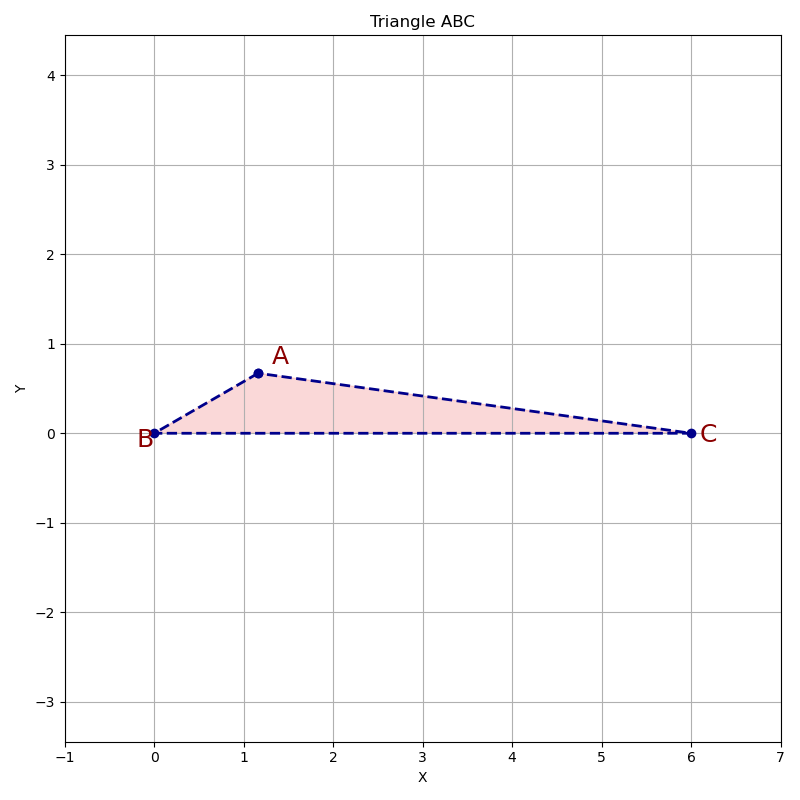
\includegraphics[width=\linewidth]{figs/fig.png}
\end{figure}
\end{frame}

\section{C Code}
\begin{frame}[fragile]
\frametitle{C Code}
\begin{lstlisting}[language=C]
#include <stdlib.h>

typedef struct {
    double x;
    double y;
} Point;

void generate_continuous_point(double x1, double y1, double x2, double y2, double t, double *x, double *y) {
    *x = (1 - t) * x1 + t * x2; 
    *y = (1 - t) * y1 + t * y2;
}
Point* generate_triangle_points(int num_points, Point v1, Point v2, Point v3) {
    Point* points = (Point*)malloc(sizeof(Point) * num_points * 3);
    double x, y;
    
   
    \end{lstlisting}
\end{frame}
\begin{frame}[fragile]
\frametitle{C Code}
\begin{lstlisting}[language=C]
   for (int i = 0; i < num_points; i++) {
         for(int j = 0; j < 3; j++){
           double t = (double)i / (num_points - 1); 
         generate_continuous_point(v1.x, v1.y, v2.x, v2.y, t, &x, &y);
        points[j].x = x;
        points[j].y = y;
         }
    }
    return points;
}
void free_points(Point* points) {
    free(points);
}
\end{lstlisting}
\end{frame}
\section{Python code}
\begin{frame}[fragile]
\frametitle{Python Code for Plotting}
\begin{lstlisting}[language=Python]
import ctypes
import matplotlib.pyplot as plt

lib = ctypes.CDLL("./generate_points.so")  
class Point(ctypes.Structure):
    _fields_ = [("x", ctypes.c_double), ("y", ctypes.c_double)]
lib.generate_triangle_points.restype = ctypes.POINTER(Point)
lib.generate_triangle_points.argtypes = [ctypes.c_int, Point, Point, Point]

num_points = 9999
v1, v2, v3 = Point(1.161, 0.671), Point(0.0, 0.0), Point(6.0, 0.0)
points = lib.generate_triangle_points(num_points, v1, v2, v3)
x_coords = [points[i].x for i in range(num_points)]
y_coords = [points[i].y for i in range(num_points)]
lib.free_points(points)
plt.figure(figsize=(8, 8))
\end{lstlisting}
\end{frame}
\begin{frame}[fragile]
\frametitle{Python Code for Plotting}
\begin{lstlisting}[language=Python]
plt.plot([v1.x, v2.x, v3.x, v1.x], [v1.y, v2.y, v3.y, v1.y], 'o--', color='darkblue', linewidth=2)
plt.fill([v1.x, v2.x, v3.x], [v1.y, v2.y, v3.y], color='lightcoral', alpha=0.3)

plt.text(v1.x + 0.15, v1.y + 0.1, 'A', fontsize=18, color='darkred')
plt.text(v2.x - 0.2, v2.y - 0.15, 'B', fontsize=18, color='darkred')
plt.text(v3.x + 0.1, v3.y - 0.1, 'C', fontsize=18, color='darkred')

plt.xlabel("X")
plt.ylabel("Y")
plt.title("Triangle ABC")
plt.grid(True)
plt.axis("equal")
plt.xlim(-1, 7)
plt.ylim(-1, 2)
plt.tight_layout()
plt.show()
\end{lstlisting}
\end{frame}


\end{document}